% -*- Mode:TeX -*-

%% IMPORTANT: The official thesis specifications are available at:
%%            http://libraries.mit.edu/archives/thesis-specs/
%%
%%            Please verify your thesis' formatting and copyright
%%            assignment before submission.  If you notice any
%%            discrepancies between these templates and the 
%%            MIT Libraries' specs, please let us know
%%            by e-mailing thesis@mit.edu

%% The documentclass options along with the pagestyle can be used to generate
%% a technical report, a draft copy, or a regular thesis.  You may need to
%% re-specify the pagestyle after you \include  cover.tex.  For more
%% information, see the first few lines of mitthesis.cls. 

%\documentclass[12pt,vi,twoside]{mitthesis}
%%
%%  If you want your thesis copyright to you instead of MIT, use the
%%  ``vi'' option, as above.
%%
%\documentclass[12pt,twoside,leftblank]{mitthesis}
%%
%% If you want blank pages before new chapters to be labelled ``This
%% Page Intentionally Left Blank'', use the ``leftblank'' option, as
%% above. 
\def\college{Caan Institute for Advanced Study}
\documentclass[12pt,twoside]{cuthesis}
\def\mystretch{2}	
\usepackage{lgrind}
%% These have been added at the request of the MIT Libraries, because
%% some PDF conversions mess up the ligatures.  -LB, 1/22/2014
\usepackage{cmap}
\usepackage{graphicx}
\usepackage{textcomp}
\usepackage{tikz}
\usepackage{pgfplots}
\pgfplotsset{width=10cm,compat=1.9} 
\usepackage{fancyhdr}
\usepackage{tikz-3dplot}
\usetikzlibrary{tikzmark}
\usepgfplotslibrary{external}
\usetikzlibrary{positioning}
\usepackage{amssymb}
\usepackage{amsmath}
\usepackage{amsfonts}
\graphicspath{ {images/} }
\usepackage[T1]{fontenc}
\pagestyle{plain}

%% This bit allows you to either specify only the files which you wish to
%% process, or `all' to process all files which you \include.
%% Krishna Sethuraman (1990).

%\typein [\files]{Enter file names to process, (chap1,chap2 ...), or `all' to
%process all files:}
%\def\all{all}
%\ifx\files\all \typeout{Including all files.} \else \typeout{Including only \files.} \includeonly{\files} \fi
\fancyfoot{}
\fancyhead[RO,LE]{\thepage}
\fancyhead[LO]{\leftmark}
\fancyhead[RE]{\rightmark}

\begin{document}
% -*-latex-*-
% 
% For questions, comments, concerns or complaints:
% thesis@mit.edu
% 
%
% $Log: cover.tex,v $
% Revision 1.8  2008/05/13 15:02:15  jdreed
% Degree month is June, not May.  Added note about prevdegrees.
% Arthur Smith's title updated
%
% Revision 1.7  2001/02/08 18:53:16  boojum
% changed some \newpages to \cleardoublepages
%
% Revision 1.6  1999/10/21 14:49:31  boojum
% changed comment referring to documentstyle
%
% Revision 1.5  1999/10/21 14:39:04  boojum
% *** empty log message ***
%
% Revision 1.4  1997/04/18  17:54:10  othomas
% added page numbers on abstract and cover, and made 1 abstract
% page the default rather than 2.  (anne hunter tells me this
% is the new institute standard.)
%
% Revision 1.4  1997/04/18  17:54:10  othomas
% added page numbers on abstract and cover, and made 1 abstract
% page the default rather than 2.  (anne hunter tells me this
% is the new institute standard.)
%
% Revision 1.3  93/05/17  17:06:29  starflt
% Added acknowledgements section (suggested by tompalka)
% 
% Revision 1.2  92/04/22  13:13:13  epeisach
% Fixes for 1991 course 6 requirements
% Phrase "and to grant others the right to do so" has been added to 
% permission clause
% Second copy of abstract is not counted as separate pages so numbering works
% out
% 
% Revision 1.1  92/04/22  13:08:20  epeisach

% NOTE:
% These templates make an effort to conform to the MIT Thesis specifications,
% however the specifications can change.  We recommend that you verify the
% layout of your title page with your thesis advisor and/or the MIT 
% Libraries before printing your final copy.
\title{Scott Caan: Scott caan, scott caan scott caan}

\author{Scott Caan}
% If you wish to list your previous degrees on the cover page, use the 
% previous degrees command:
%       \prevdegrees{A.A., Harvard University (1985)}
% You can use the \\ command to list multiple previous degrees
%       \prevdegrees{B.S., University of California (1978) \\
%                    S.M., Massachusetts Institute of Technology (1981)}
\department{Department of Caan}

% If the thesis is for two degrees simultaneously, list them both
% separated by \and like this:
 \degree{Doctor of Caan}
%degree{Bachelor of Science in Computer Science and Engineering}

% As of the 2007-08 academic year, valid degree months are September, 
% February, or June.  The default is June.
\degreemonth{February}
\degreeyear{2016}
\thesisdate{September 21, 2015}

%% By default, the thesis will be copyrighted to MIT.  If you need to copyright
%% the thesis to yourself, just specify the `vi' documentclass option.  If for
%% some reason you want to exactly specify the copyright notice text, you can
%% use the \copyrightnoticetext command.  
\copyrightnoticetext{\copyright Scott Caan, 2015.}

% If there is more than one supervisor, use the \supervisor command
% once for each.
\supervisor{James Caan}{Professor, Caan Studies, Caan Institute}
\supervisor{Casey Affleck}{Professor, Affleck Department}

% This is the department committee chairman, not the thesis committee
% chairman.  You should replace this with your Department's Committee
% Chairman.
\chairman{Matt Damon}{Chair, Matt Damon}

% Make the titlepage based on the above information.  If you need
% something special and can't use the standard form, you can specify
% the exact text of the titlepage yourself.  Put it in a titlepage
% environment and leave blank lines where you want vertical space.
% The spaces will be adjusted to fill the entire page.  The dotted
% lines for the signatures are made with the \signature command.
\maketitle

% The abstractpage environment sets up everything on the page except
% the text itself.  The title and other header material are put at the
% top of the page, and the supervisors are listed at the bottom.  A
% new page is begun both before and after.  Of course, an abstract may
% be more than one page itself.  If you need more control over the
% format of the page, you can use the abstract environment, which puts
% the word "Abstract" at the beginning and single spaces its text.

%% You can either \input (*not* \include) your abstract file, or you can put
%% the text of the abstract directly between the \begin{abstractpage} and
%% \end{abstractpage} commands.

% First copy: start a new page, and save the page number.
\cleardoublepage
% Uncomment the next line if you do NOT want a page number on your
% abstract and acknowledgments pages.
% \pagestyle{empty}
\setcounter{savepage}{\thepage}
\begin{abstractpage}
% $Log: abstract.tex,v $
% Revision 1.1  93/05/14  14:56:25  starflt
% Initial revision
% 
% Revision 1.1  90/05/04  10:41:01  lwvanels
% Initial revision
% 
%
%% The text of your abstract and nothing else (other than comments) goes here.
%% It will be single-spaced and the rest of the text that is supposed to go on
%% the abstract page will be generated by the abstractpage environment.  This
%% file should be \input (not \include 'd) from cover.tex.
Scott Caan scott caan scott; caan, scott caan scott caan, Scott Caan scott caan, scott, caan scott. Scott caan, scott caan scott caan scott "caan", scott caan. Scott caan scott caan scott caan "scott caan scott", caan scott caan, scott, caan scott caan scott.
\end{abstractpage}

% Additional copy: start a new page, and reset the page number.  This way,
% the second copy of the abstract is not counted as separate pages.
% Uncomment the next 6 lines if you need two copies of the abstract
% page.
% \setcounter{page}{\thesavepage}
% \begin{abstractpage}
% % $Log: abstract.tex,v $
% Revision 1.1  93/05/14  14:56:25  starflt
% Initial revision
% 
% Revision 1.1  90/05/04  10:41:01  lwvanels
% Initial revision
% 
%
%% The text of your abstract and nothing else (other than comments) goes here.
%% It will be single-spaced and the rest of the text that is supposed to go on
%% the abstract page will be generated by the abstractpage environment.  This
%% file should be \input (not \include 'd) from cover.tex.
Scott Caan scott caan scott; caan, scott caan scott caan, Scott Caan scott caan, scott, caan scott. Scott caan, scott caan scott caan scott "caan", scott caan. Scott caan scott caan scott caan "scott caan scott", caan scott caan, scott, caan scott caan scott.
% \end{abstractpage}

\cleardoublepage

\section*{Acknowledgments}
``Into the Blue'' is my ``Ulysses''. \\\textit{Scott Caan}
%%%%%%%%%%%%%%%%%%%%%%%%%%%%%%%%%%%%%%%%%%%%%%%%%%%%%%%%%%%%%%%%%%%%%%
% -*-latex-*-

\pagenumbering{Roman} 
% Some departments (e.g. 5) require an additional signature page.  See
% signature.tex for more information and uncomment the following line if
% applicable.
% % -*- Mode:TeX -*-
%
% Some departments (e.g. Chemistry) require an additional cover page
% with signatures of the thesis committee.  Please check with your
% thesis advisor or other appropriate person to determine if such a 
% page is required for your thesis.  
%
% If you choose not to use the "titlepage" environment, a \newpage
% commands, and several \vspace{\fill} commands may be necessary to
% achieve the required spacing.  The \signature command is defined in
% the "mitthesis" class
%
% The following sample appears courtesy of Ben Kaduk <kaduk@mit.edu> and
% was used in his June 2012 doctoral thesis in Chemistry. 

\begin{titlepage}
\begin{large}
This doctoral thesis has been examined by a Committee of the Department
of Chemistry as follows:

\signature{Professor Jianshu Cao}{Chairman, Thesis Committee \\
   Professor of Chemistry}

\signature{Professor Troy Van Voorhis}{Thesis Supervisor \\
   Associate Professor of Chemistry}

\signature{Professor Robert W. Field}{Member, Thesis Committee \\
   Haslam and Dewey Professor of Chemistry}
\end{large}
\end{titlepage}


%\pagestyle{plain}
\pagestyle{fancy}
\setlength{\headheight}{15pt} 
  % -*- Mode:TeX -*-
%% This file simply contains the commands that actually generate the table of
%% contents and lists of figures and tables.  You can omit any or all of
%% these files by simply taking out the appropriate command.  For more
%% information on these files, see appendix C.3.3 of the LaTeX manual. 
\tableofcontents
\newpage
\listoffigures
\newpage
\listoftables


% chap1 = Intro, specific aims, scott caan
\pagenumbering{arabic} 
%% This is an example first chapter.  You should put chapter/appendix that you
%% write into a separate file, and add a line \include{yourfilename} to
%% main.tex, where `yourfilename.tex' is the name of the chapter/appendix file.
%% You can process specific files by typing their names in at the 
%% \files=
%% prompt when you run the file main.tex through LaTeX.
\chapter{Introduction}

\section{Motivations}

\begin {figure}[htbp]
\centering
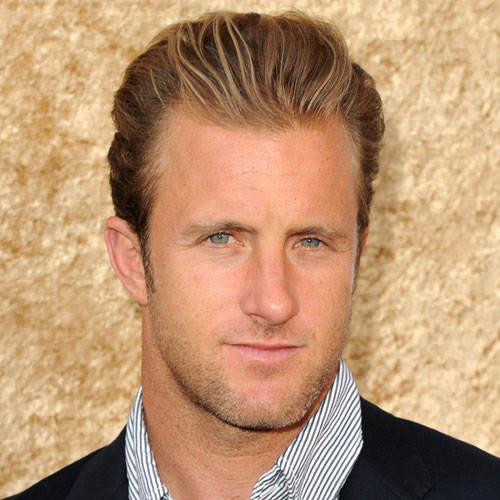
\includegraphics[width=\textwidth]{scottcaan1}
\caption{Scott Caan}
\label{fig1}
\centering
\end{figure}
\subsection{Specific aim 1: Scott Caan }

        	Scott Caan, scott caan scott caan scott caan? Scott "caan" scott caan scott "caan": scott caan, scott caan scott, caan scott caan scott. Scott caan scott.
\subsection{Specific Aim 2: Scott Caan}

Scott caan scott caan scott caan. Scott "caan", scott caan scott\cite{caan1}, caan scott, caan scott.
 
\begin {figure}[htbp]
\centering
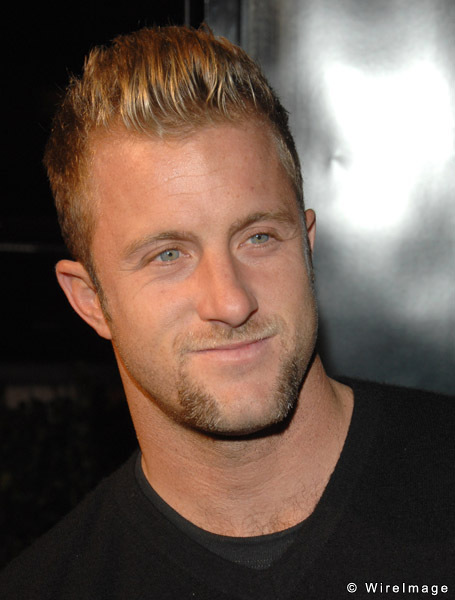
\includegraphics[scale=.5]{scottcaan2}
\caption{Scott Caan}
\label{fig2}
\centering
\end{figure}

 
\subsection {Specific aim 3: Scott Caan}

Scott caan, scott caan scott, caan\cite{caan2} "scott caan", scott caan. Scott caan; scott, caan, scott, caan scott. 

\section{Innovation}
Scott caan? Scott caan.
\begin {figure}[htbp]
\centering
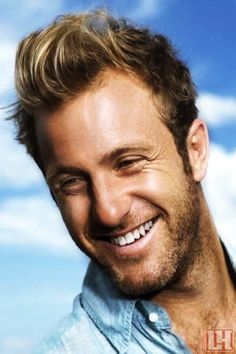
\includegraphics[scale=0.5]{scottcaan3}
\caption{Scott Caan}
\label{fig3}
\centering
\end{figure}

\section{Background}

\subsection{Scott Caan}
	Scott caan scott. Scott caan scott caan scott: caan scott caan.
\subsection{Scott Caan}
	Scott caan scott? Caan scott caan scott. Caan scott caan scott, caan scott. 
\begin {figure}[htbp]
\centering
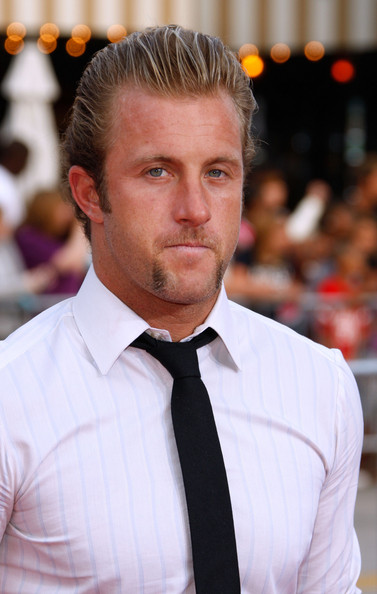
\includegraphics[scale=.5]{scottcaan4}
\caption{Scott Caan}
\label{fig4}
\centering
\end{figure}

Scott caan scott caan scott caan scott, caan scott caan.\cite{caan3} "Scott Caan", scott caan scott caan. Scott Caan.
 

\subsection{Abbreviations}
\textbf{SC} Scott Caan

% chap2 = Scott Caan
%% This is an example first chapter.  You should put chapter/appendix that you
%% write into a separate file, and add a line \include{yourfilename} to
%% main.tex, where `yourfilename.tex' is the name of the chapter/appendix file.
%% You can process specific files by typing their names in at the 
%% \files=
%% prompt when you run the file main.tex through LaTeX.
%   _____ ______      __  _____             
%  / ____|  _ \ \    / / |  __ \            
% | |    | |_) \ \  / /  | |  | | _____   __
% | |    |  _ < \ \/ /   | |  | |/ _ \ \ / /
% | |____| |_) | \  /    | |__| |  __/\ V / 
%  \_____|____/   \/     |_____/ \___| \_/  
%                                           
%                                           

\chapter{Specific Aim 1: Scott Caan}

\section{Scott Caan}

\subsection{Introduction and study design}
 Scott Caan?\cite{caan4}
\subsection{Methods}
\begin {figure}[htbp]
\centering
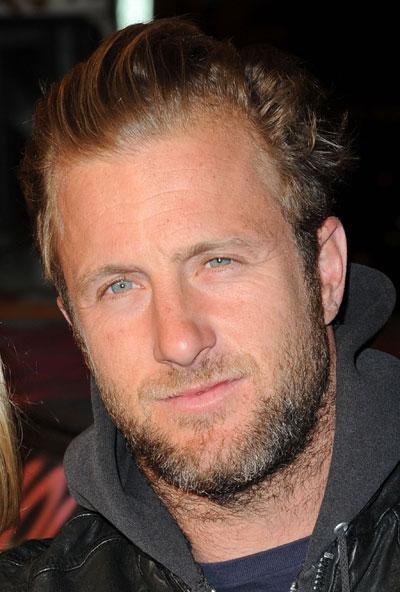
\includegraphics[scale=.5]{scottcaan5}
\caption{Scott Caan}
\label{fig5}
\centering
\end{figure}
Scott Caan...
\subsection{Results and discussion}


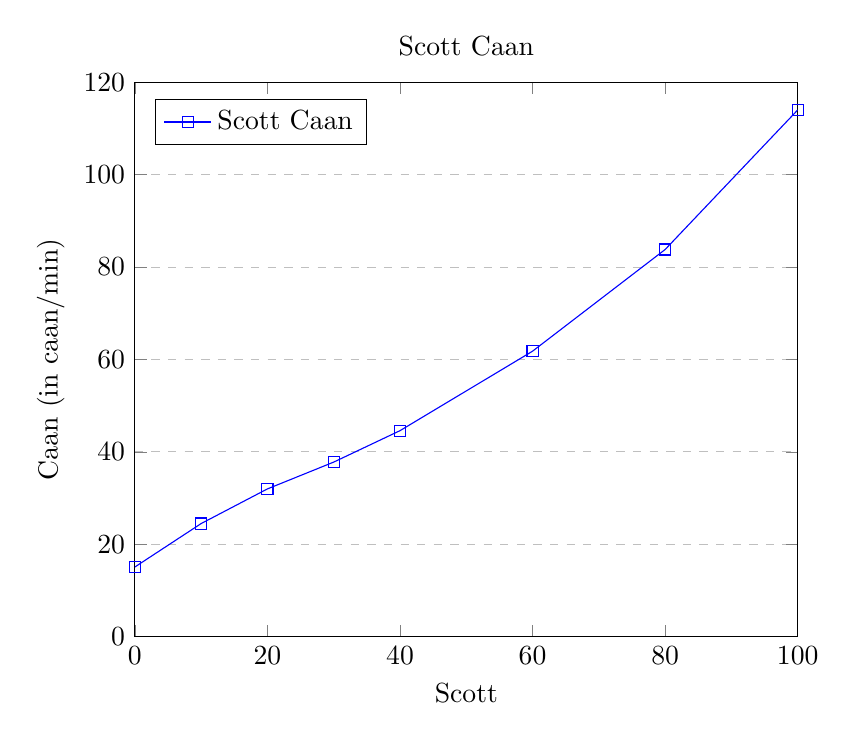
\begin{tikzpicture}
\begin{axis}[
    title={Scott Caan},
    xlabel={Scott},
    ylabel={Caan (in caan/min)},
    xmin=0, xmax=100,
    ymin=0, ymax=120,
    xtick={0,20,40,60,80,100},
    ytick={0,20,40,60,80,100,120},
    legend pos=north west,
    ymajorgrids=true,
    grid style=dashed,
]
 
\addplot[
    color=blue,
    mark=square,
    ]
    coordinates {
    (0,15.1)(10,24.5)(20,32)(30,37.8)(40,44.6)(60,61.8)(80,83.8)(100,114)
    };
    \legend{Scott Caan}
 
\end{axis}
\end{tikzpicture}



Scott Caan.
\subsection{Conclusion}
Scott Caan!\cite{caan5}
% chap3 = Scott Caan

\pagestyle{plain}
\appendix
\chapter{Appendix}
\begin{table}[]
\centering
\caption{Scott Caan}
\label{table1}
\begin{tabular}{ll}
Actor                    & Boolean \\
Scott Caan          & TRUE    \\
Greogory Peck    & FALSE  
\end{tabular}
\end{table}

%% This defines the bibliography file (main.bib) and the bibliography style.
%% If you want to create a bibliography file by hand, change the contents of
%% this file to a `thebibliography' environment.  For more information 
%% see section 4.3 of the LaTeX manual.
\begin{singlespace}
\bibliography{main.bib}
\bibliographystyle{plainnonote}
\end{singlespace}

\end{document}

